
\chapter{Peletizadora}
\label{ane:peletizadora}

Algo que no se tuvo en cuenta al establecer los objetivos del proyecto, fue el tener disponibilidad de pellets de PLA, ya que en ese momento, los pellets no los proporcionarían PESL para poder hacer las pruebas de la puesta en marcha. Por ello, se investiga en la posibilidad de reciclar bobinas defectuosas que no son útiles para imprimir en una impresora 3D ocasionando averias y en la actualidad son mermas que se tiene en la producción de la fábrica de Huesca PESL.

\begin{figure}[H]
    \centering
    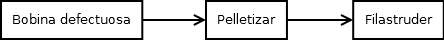
\includegraphics[width=0.6\textwidth]{images/peletizadora/Diagram.png}
    \caption{Proceso para conseguir pellets}
    \label{fig:peletizadora_diagram}
\end{figure}

Una vez que la filastruder está operativa, se peletizan a mano unos metros de filamento negro y comprobamos que al menos somos capaces de extruir los pellets reciclados. Se continua con la línea de investigación del reciclado de bobina as al comprobar la viabilidad del proceso. Sin embargo, cada bobina de filamento de 1Kg de peso son 350M por lo que peletizar una bobina a mano, conllevaría mucho tiempo y trabajo, por lo que se descarta la opción y se pasa a diseñar una máquina capaz de peletizar bobinas de forma automática. La máquina que diseñemos debe ser capaz de realizar el siguiente proceso:

\begin{figure}[H]
    \centering
    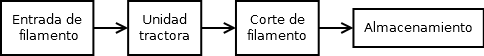
\includegraphics[width=0.6\textwidth]{images/peletizadora/Diagram2.png}
    \caption{Proceso funcionamiento peletizadora}
    \label{fig:peletizadora_diagram2}
\end{figure}

Por tanto, debe tener al menos dos partes diferenciadas:

\begin{itemize}
	\item{\textbf{Unidad Tractora:} Mecanismo capaz de arrastrar el filamento hacía la unidad de corte.}
	\item{\textbf{Cuchillas de corte:} Mecanismo capaz de ejercer la fuerza necesaria para cortar el filamento.}
\end{itemize}

Para controlar toda la máquina se decide usar una placa arduino Mega que se tiene disponible en el departamento, con la que seremos capaz de controlarlo. Para la fabricación de la máquina, se usarán impresoras 3D, con lo que el prototipado será más rápido, ya que se tiene acceso a ellas dentro del departamento. Con las herramientas disponibles se inicia el diseño de la máquina.\\

Para la unidad tractora, se deciden usar dos motores paso a paso con un eje de giro recubierto de una goma, que cogerá el filamento y lo arrastrará. Usando la herramienta Inventor, se hace un primer diseño de la posible solución.

\begin{figure}[H]
    \centering
    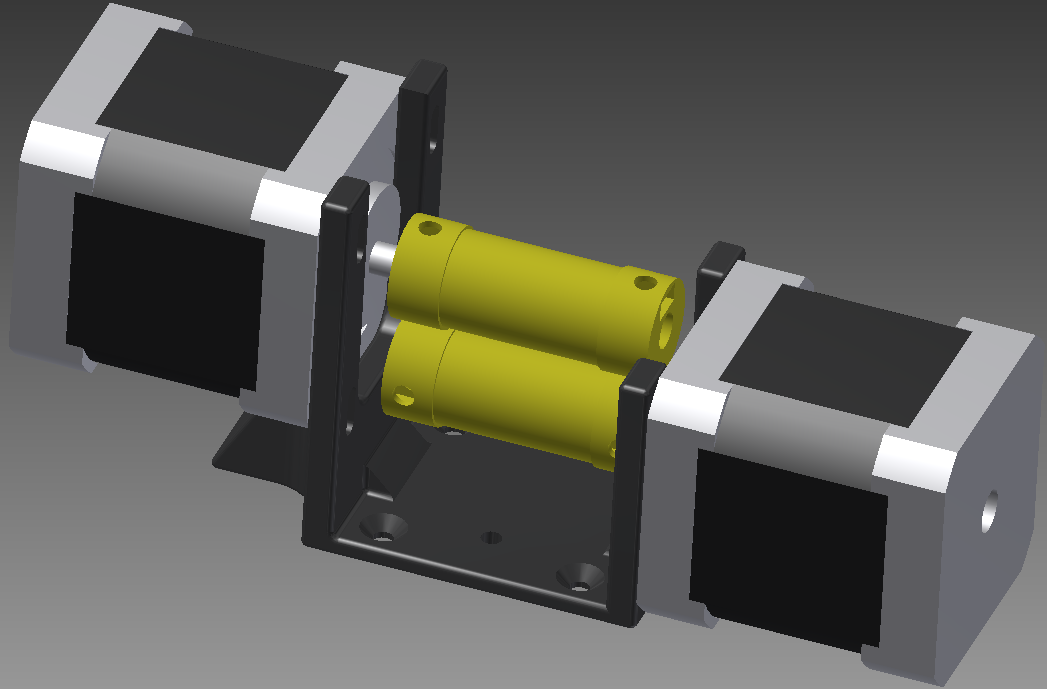
\includegraphics[width=0.6\textwidth]{images/peletizadora/unidadtractora.png}
    \caption{Diseño de la unidad tractora}
    \label{fig:peletizadora_tractora}
\end{figure}

Los ejes, deberán ir recubiertos de goma de neopreno, para que puedan arrastrar del filamento. Se eligen motores paso a paso, debido a:

\begin{itemize}
	\item{Fáciles de programar.}
	\item{Fáciles de controlar en velocidad.}
	\item{Gran fuerza neta en el eje.}
\end{itemize}

Aunque el mecanismo es capaz de tirar del filamento bobinado, es necesario que se le guíe para que el corte sea siempre en la misma posición, por tanto, se diseña una guía para que la salida del filamento sea siempre por el mismo sitio, a la pieza impresa, se le pondrá una plancha de metal para que al realizar el corte, el filamento se apoye sobre ella y se ejerza más fuerza a cizalla. Además, deberá tener forma de embudo, para que la entrada del filamento sea lo más amplia posible y el final sea un único cilindro de un tamaño similar al del diámetro de filamento:

\begin{figure}[H]
    \centering
    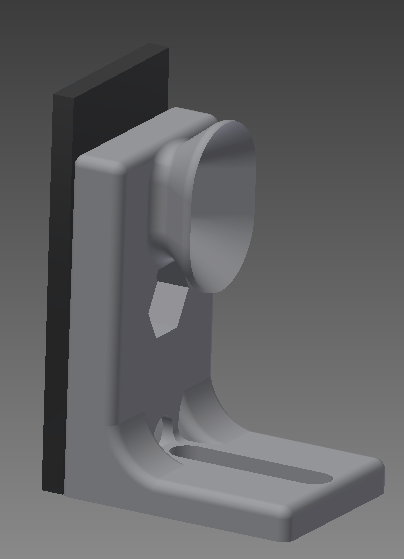
\includegraphics[width=0.4\textwidth]{images/peletizadora/guia.png}
    \caption{Diseño de guía de filamento}
    \label{fig:peletizadora_guia}
\end{figure}

El diseño final de la unidad tractora se ve a continuación:

\begin{figure}[H]
    \centering
    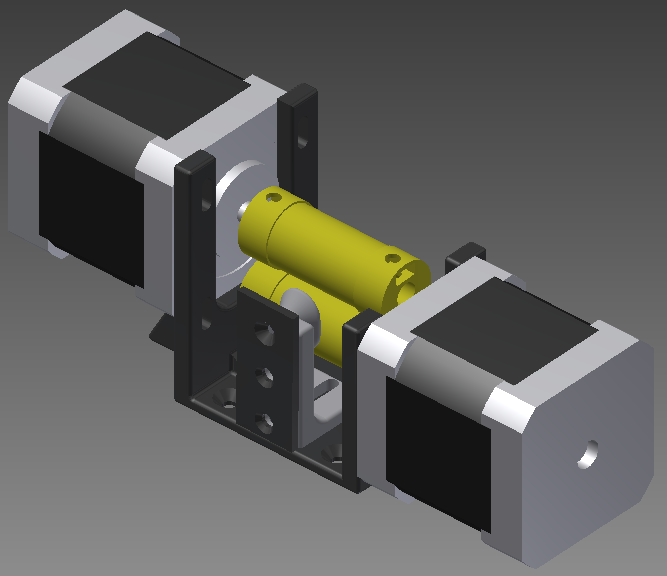
\includegraphics[width=0.5\textwidth]{images/peletizadora/conjunto_tractora.png}
    \caption{Conjunto tractora completo}
    \label{fig:peletizadora_conjunto}
\end{figure}

Con este conjunto, garantizamos que el desbobinado del filamento sea correcto, aparte, seremos capaces de regular la velocidad de tracción de forma controlada. El siguiente paso a realizar será el diseño de las cuchillas de corte.\\

Como unidad motriz de las cuchillas de corte, se elige un taladro con fuerza ajustable, en la boca del mismo, se acoplará un eje con las cuchillas. Como primera idea, se piensa en un diseño con un molino a cuatro ejes, donde en cada uno de ellos irá una cuchilla, de esta manera, por cada giro se podrán realizar cuatro cortes.

\begin{figure}[H]
    \centering
    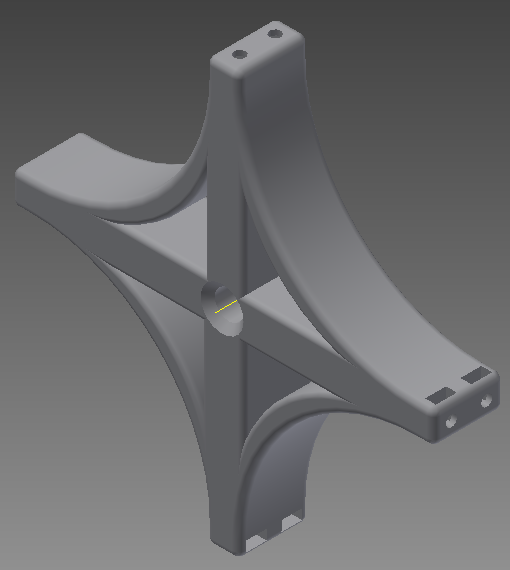
\includegraphics[width=0.4\textwidth]{images/peletizadora/aspas.png}
    \caption{Diseño de las aspas}
    \label{fig:peletizadora_aspas}
\end{figure}

El conjunto de las aspas, irán instaladas sobre dos pilares, que harán de eje de giro al taladro, a su vez, se instalará una rampa de salida, para que los pellets vayan cayendo por ella, por último, para tapar todas las cuchillas y añadir seguridad al mecanismo, se incorpora una tapa que hará que las cuchillas no sean accesibles.

\begin{figure}[H]
    \centering
    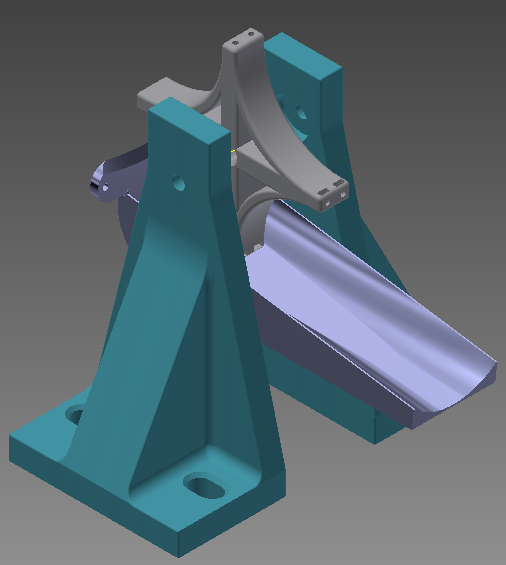
\includegraphics[width=0.4\textwidth]{images/peletizadora/corte.png}
    \caption{Mecanismo de corte}
    \label{fig:peletizadora_corte}
\end{figure}

Una vez impresas todas las piezas y realizado el montaje se realizan pruebas del mecanismo, se detecta que el filamento es capaz de desgastar la goma del eje de los motores, por ello, se incorpora a la entrada de la tracción un servo que hace que el filamento oscile, haciendo que el desgaste de la goma sea menor.

\begin{figure}[H]
    \centering
    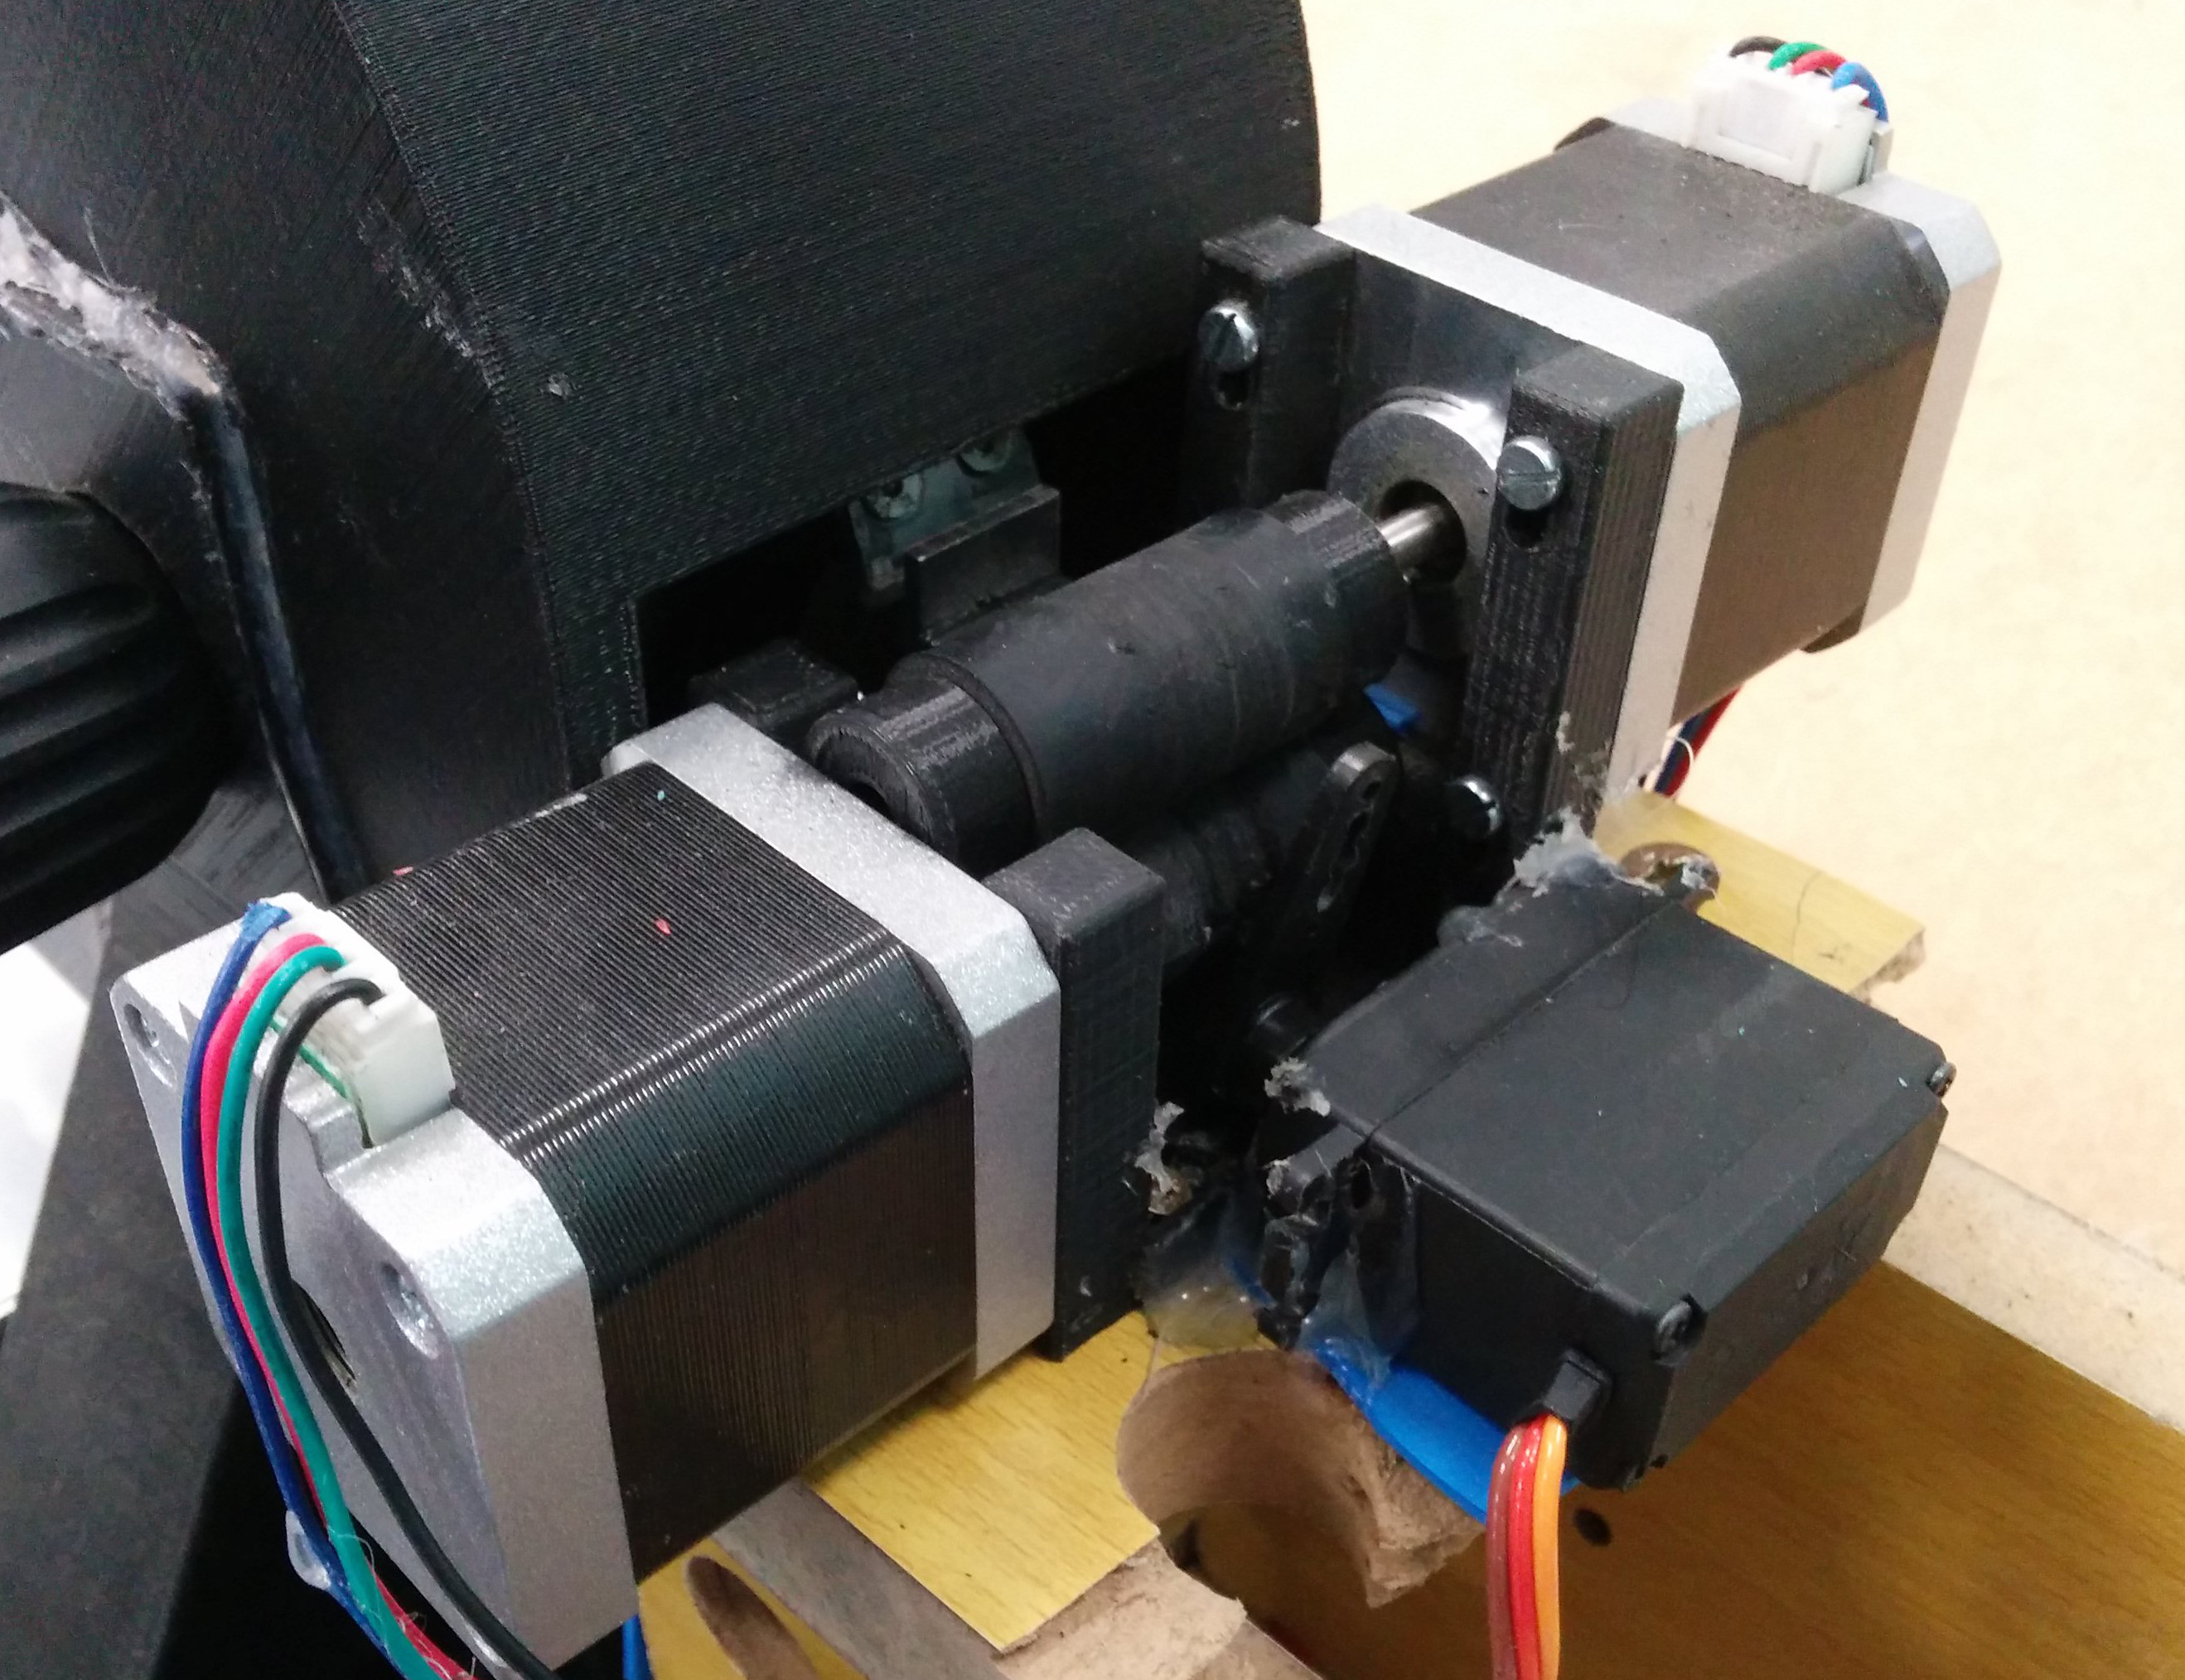
\includegraphics[width=0.4\textwidth]{images/peletizadora/IMG_20150818_172903.jpg}
    \caption{Mecanismo impreso con servo para generar oscilación}
    \label{fig:peletizadora_mecanismo}
\end{figure}

\begin{figure}[H]
    \centering
    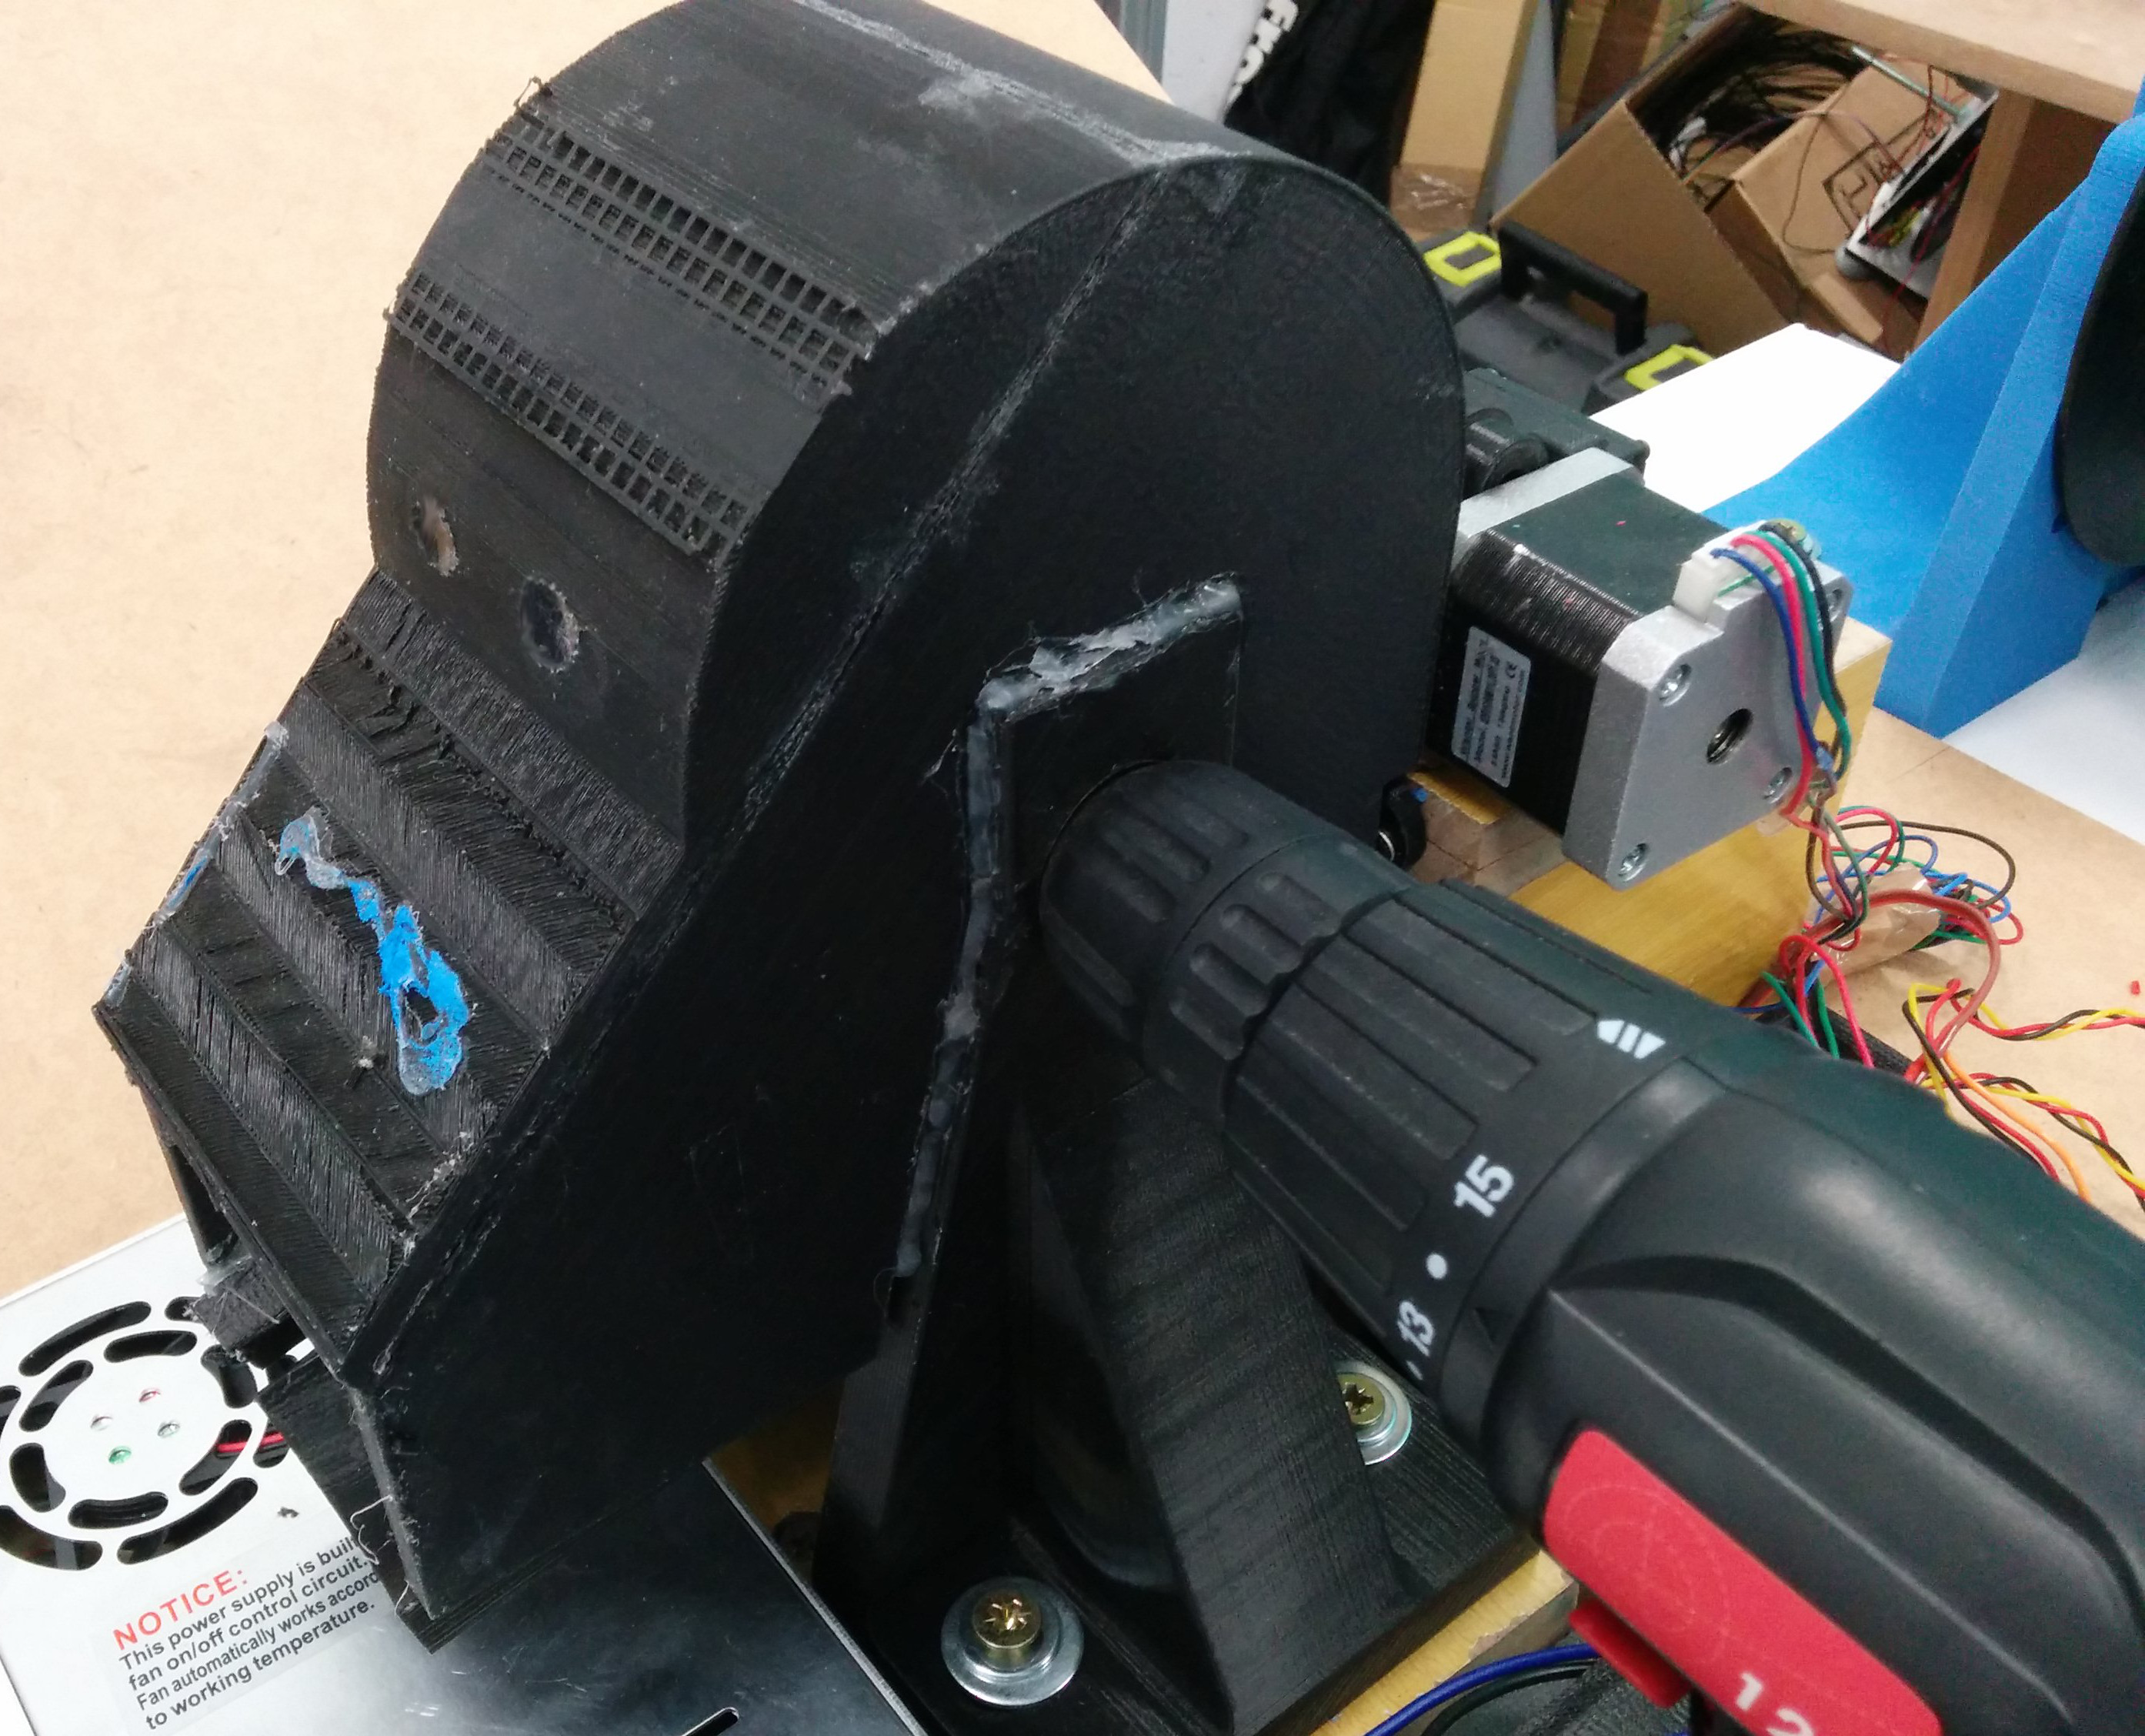
\includegraphics[width=0.4\textwidth]{images/peletizadora/IMG_20150818_172917.jpg}
    \caption{Estructura con aspas encerradas.}
    \label{fig:peletizadora_mecanismo2}
\end{figure}

Una vez el diseño se da por bueno, somos capaces de peletizar una bobina de 1 Kg en 30 minutos con una longitud del pellet de 0.5 mm. Por tanto, el problema de conseguir pellets para extruir lo hemos solucionado. Más adelante, se realizará un ensayo de calorimetría de barrido diferencial (DSC) con la que analizaremos térmicamente el filamento extruido en la filastruder, y comprobaremos la degradación que ha sufrido el polímero.
    
\begin{figure}[H]
    \centering
    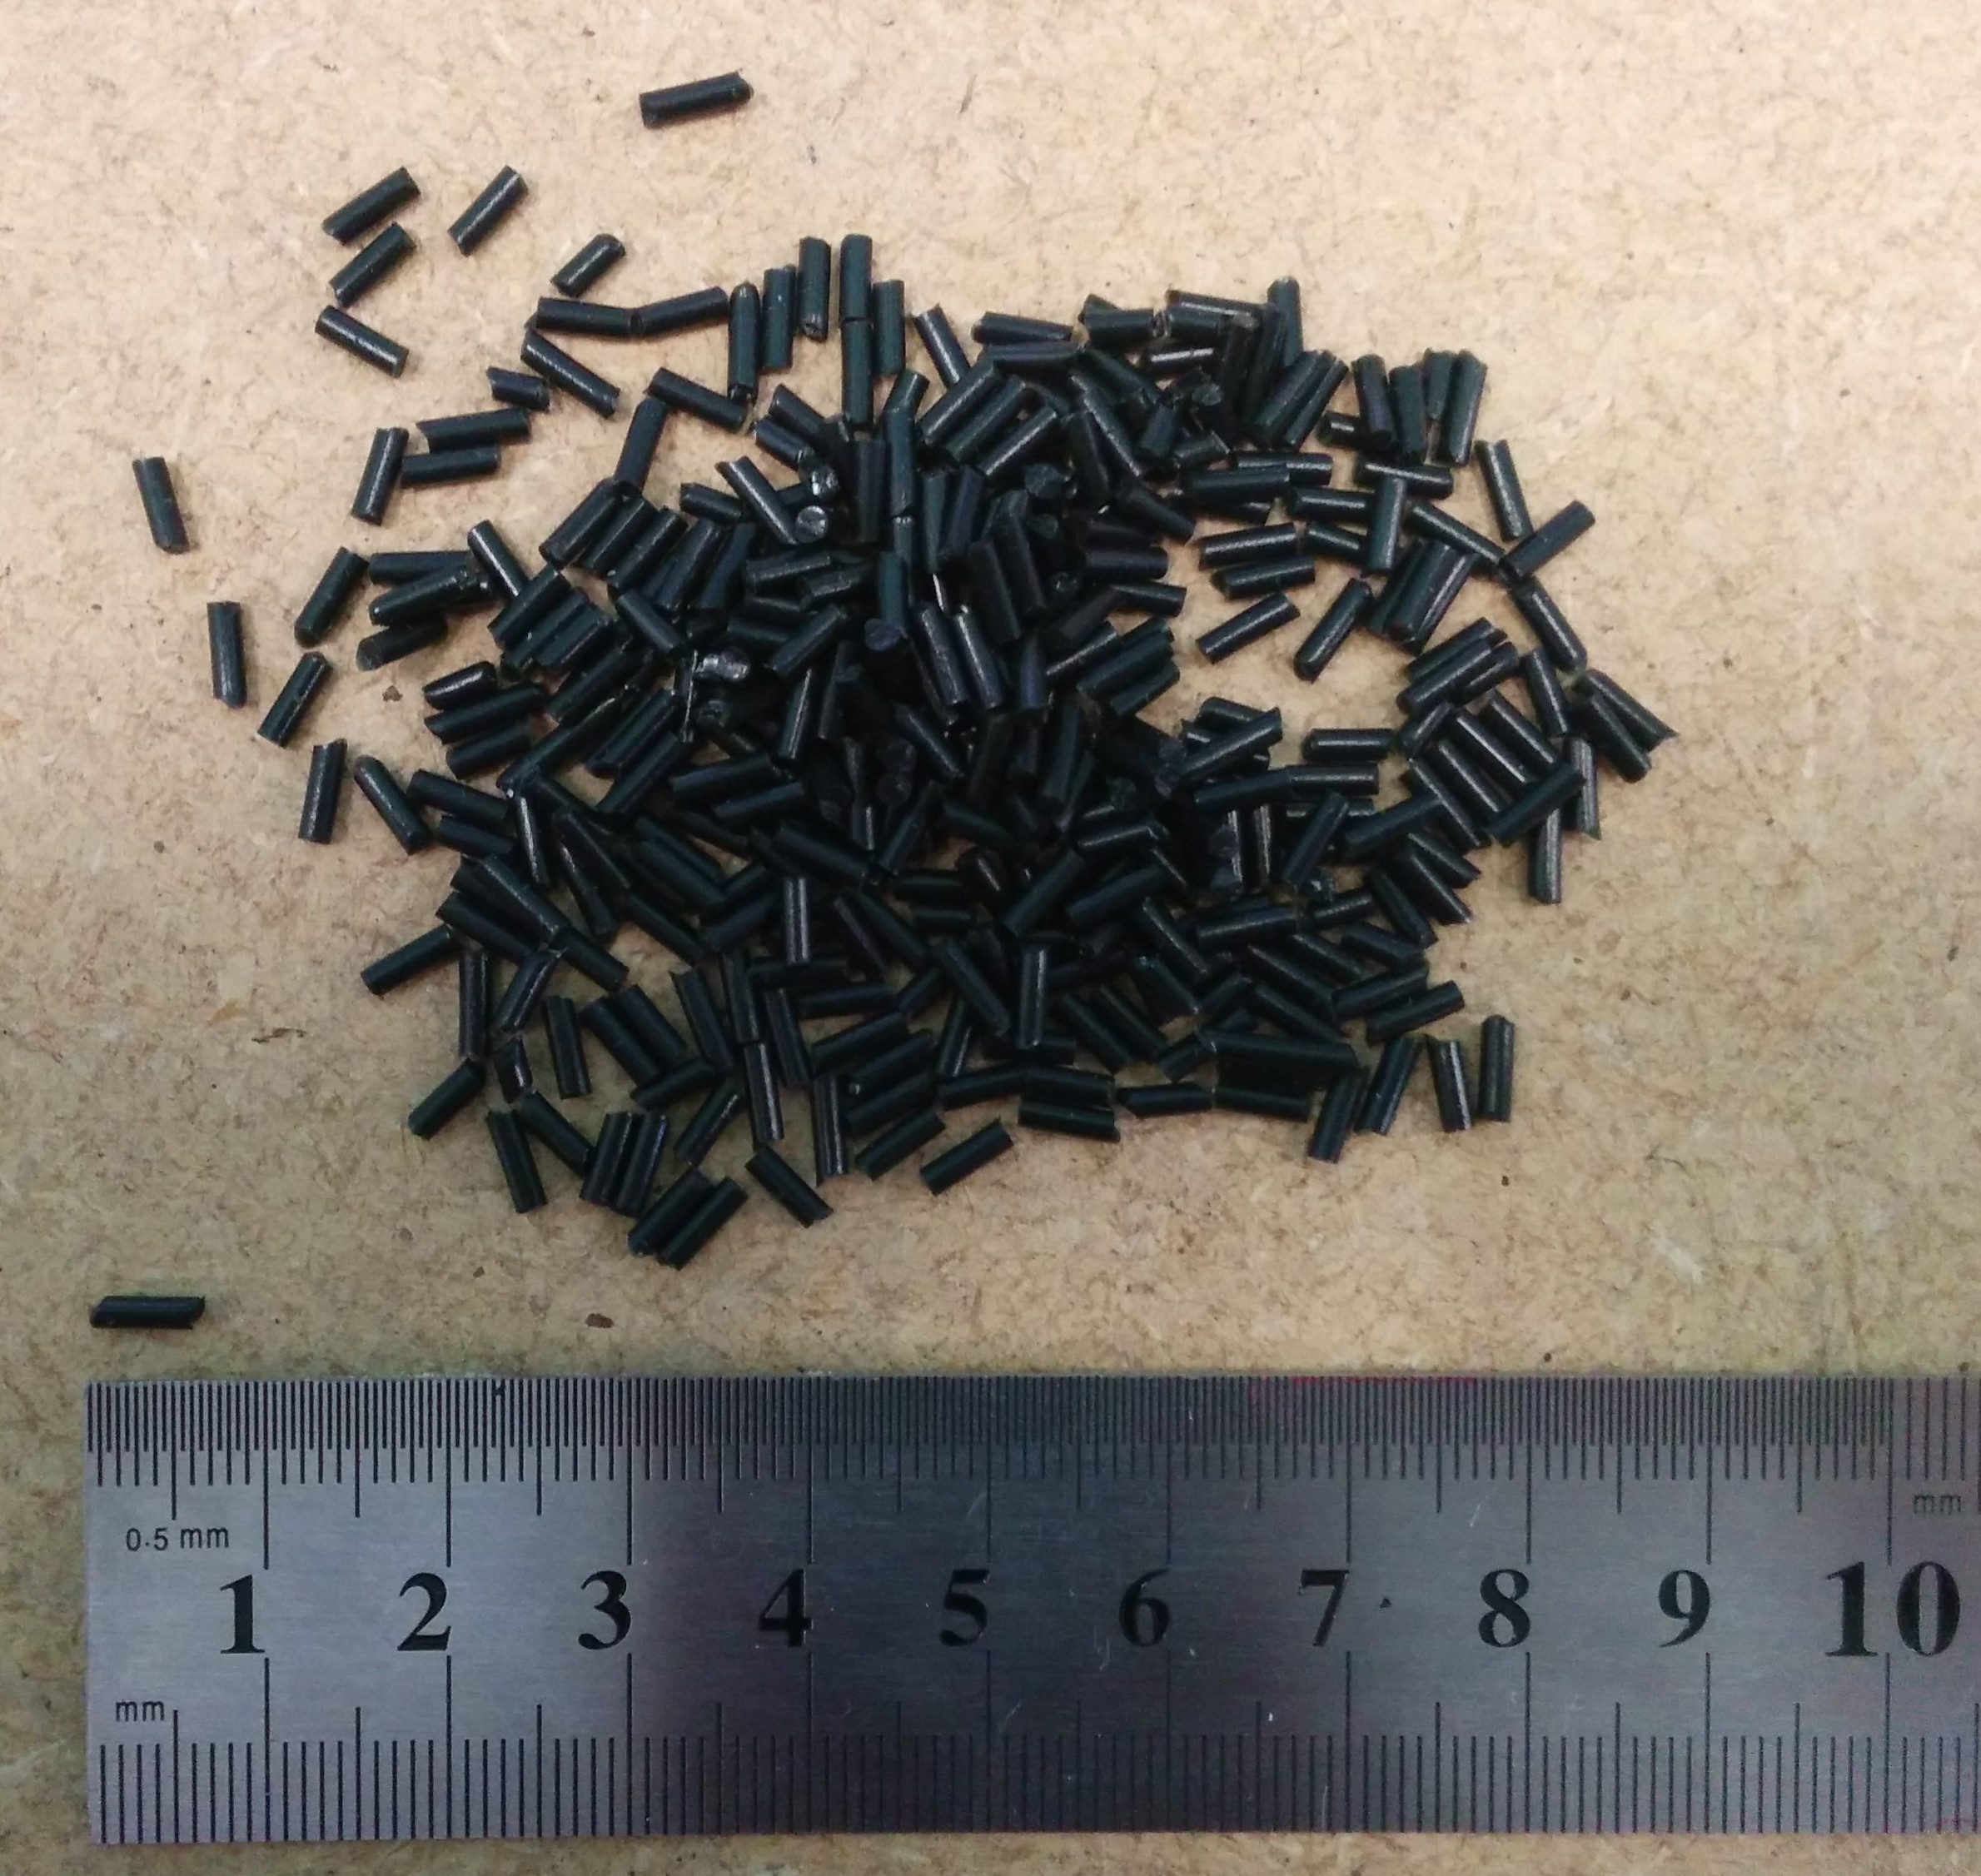
\includegraphics[width=0.3\textwidth]{images/peletizadora/IMG_20150819_112740.jpg}
    \caption{Pellets de filamento reciclado.}
    \label{fig:peletizadora_pellets_reciclados}
\end{figure}